\documentclass[format=sigconf]{acmart}

\usepackage{algorithm}
\usepackage{algorithmic}
\usepackage{booktabs}
\usepackage{hyperref}

\begin{document}

\title{CSE-6140 Final Project}
\author{Filip Gajowniczek}
\author{Nick Dargi}

% This template is probably useful
% https://www.overleaf.com/latex/templates/acm-conference-proceedings-master-template/pnrfvrrdbfwt

\section{Introduction}
The Traveling Salesman Problem (TSP) is an NP-Complete computational problem which has been studied extensively for several decades \cite{laporte_1992}. In this paper, techniques for obtaining/approximating the solution to the symmetric Traveling Salesman Problem are developed and compared. 
A branch-and-bound algorithm using a minimum spanning tree to inform a lower bound on sub-problems is presented; which, given enough time, produces an exact solution to the problem. The use of approximation algorithms proves more prudent for larger problems while sacrificing solution quality; a fact which motivated the development of a greedy local search algorithm which explores 1-exchange neighbors. 
In addition, two local search algorithms a 2-Opt Hill Climb and Simulated Annealing Algorithm are explored. 
These local search algorithms are ideal for finding low error solutions in limited time, although no performance bounds are guaranteed beyond 
what is expected from the Greedy Algorithms that initially seed them. The results derived showed that the local search algorithms were 
extremely adept at providing relatively good solutions even in the presence of large data sets, however they struggled to consistently return optimal solutions even for the smaller 
data-sets. Of the two local search algorithms explored, the simulated annealing algorithm provided clear benefits especially for larger data sets which contain a higher number of local optima which can frequently trap
 other algorithms in a non optimal neighborhood. \textit{Note: For the purposes of this project the Simulated Annealing 
 and Approximation Algorithms are considered to be the two primary algorithms for scoring purposes, with the Branch-and-Bound and 
 2-OPT Hill Climb serving as the extra credit algorithms.}
\section*{Problem Definition}
The symmetric traveling salesman optimization problem is formalized as follows:\\
Given a connected undirected graph G consisting of n nodes,$\{v_0, \hdots, v_{n-1}\}$ , with edge weights $d_{ij}$ between nodes i and j.
Find a Hamiltonian Cycle, a path P* where each node has degree 2, with minimum weight.\\
In this paper, nodes in a 2 dimensional space were considered: $v_i = \begin{bmatrix}
v_{ix} \\ v_{iy} 
\end{bmatrix} \in \mathbb{R}^2 \quad \forall i \in [0,n-1]$\\
With edge weights calculated using the Euclidean distance: $e_{ij} = || v_i, v_j ||_2 = \sqrt{(v_{ix}-v_{jx})^2 + ((v_{iy}-v_{jy}^2)} \quad \forall i\neq j, i \in [0,n-1], j \in [0,n-1]$\\
The solution is an element in the set of vertex sequences which are Hamiltonian Cycles given by:\\
$\mathcal{H} = \{ (v_i)_{i=0}^{n-1} : v_0 = v_{n-1}, v_i \neq v_j \quad \forall i,j \in [0,n-1]\}$\\
The symmetric TSP is given by following optimization problem:\\ 
$P^*=(v^*_i)_{i=0}^{n-1} =\quad  \stackrel{argmin}{(v_i)_{i=0}^{n-1} \in \mathcal{H}} \quad \sum_{i=0}^{n-2} ||v_i, v_{i+1} || + ||v_0, v_{n-1} || $
\section*{Related Work}
The Traveling Salesman Problem has been a widely studied in the fields of graph theory and computational 
algorithms for almost 200 years. Long considered impossible, formal methods for restricting the problem space using 
approximation algorithms, similar to the 2MST approximation used here. With formal methods to approximate routes to given accuracies solving the problem 
for large data-sets became feasible in practice. With a good starting point for lower bounds, methods such as the Branch-and-Bound method used in this paper 
could now solve large data-sets by limiting the search space using the previously calculated lower bounds given by the approximation guarantee. Recently in 2011 
researchers from Stanford and McGill Universities were able to improve upon the approximation algorithm developed by Nicos Christofides 
in 1976 which had defined performance bounds of at most 50\% greater than the true optimal solution when they developed an approximation technique 
which improved upon Christofides' algorithm by four hundredths of a trillionth of a trillionth of a trillionth of a trillionth of a percent, a staggeringly small 
value in most other scenarios. Although this improvement was relatively minimal, it broke open a wall that existed in the world of computer science for over 35 years, proving 
that in practice a better solution was possible. With the rise of Quantum Computing improved results for the Traveling Salesman Problem will not only be made possible by improved algorithms, 
but also by the exponential increase in processing power that the Quantum Technology brings. With this technology on the rise we are poised to see major improvements in the runtime of NP-Hard algorithms such as the TSP 
problem which will be extremely important given the increase in the use of Big Data throughout virtually every industry. \cite{CS_Sci}
\section*{Algorithms}
\begin{algorithm}[H] 
	\caption{  BnB( $\{v_0, \hdots, v_{n-1}\}$ ): Find minimum cost Hamiltonian Cycle for euclidean distances}
	\begin{algorithmic} 
		\STATE Data: $\{v_0, \hdots, v_{n-1}\}$ set of 2-D points
		\FORALL{ Unordered Pairs $\{i,j\}$}
			\STATE Construct edge $e = (v_i, v_j, d_{ij})$
			\STATE Add e to list E of edges in increasing weight order: $E = E \cup \{e\}$
		\ENDFOR
	\end{algorithmic}
\end{algorithm}
\begin{algorithm}[H] 
	\caption{  2-Opt\_HC( $\{v_0, \hdots, v_{n-1}\}$ ): Approximate the minimum cost Hamiltonian Cycle for euclidean distances using a Hill Climbing local search algorithm with 2-Opt exchange Neighborhood Creation}
	\begin{algorithmic} 
		\STATE Data: $\{v_0, \hdots, v_{n-1}\}$ set of 2-D points
		\FORALL{ Unordered Pairs $\{i,j\}$}
			\STATE Construct edge $e = (v_i, v_j, d_{ij})$
			\STATE Add e to list E of edges in increasing weight order: $E = E \cup \{e\}$
		\ENDFOR
		\WHILE{Unassigned nodes in $v$}
			\STATE Assign Nodes to Route based on Greedy Nearest Neighbor implementation
		\ENDWHILE
		\FOR{$i = 1$ to length(Route Matrix)}
			\FOR{$j = i+1$ to length(Route Matrix)}
				\STATE reverse array (route[i] to route[j]) and add it to newroute[i] to newroute[j]
				\IF{cost(newroute) < cost(route)}
					\STATE route $\leftarrow$ newroute
				\ENDIF
			\ENDFOR
		\ENDFOR

	\end{algorithmic}
\end{algorithm}

\begin{algorithm}[H] 
	\caption{  Sim\_Anneal( $\{v_0, \hdots, v_{n-1}\}$ ): Approximate the minimum cost Hamiltonian Cycle for euclidean distances using a Hill Climbing local search algorithm with 2-Opt exchange Neighborhood Creation}
	\begin{algorithmic} 
		\STATE Data: $\{v_0, \hdots, v_{n-1}\}$ set of 2-D points
		\STATE Current\_Route: $\{c_0, \hdots, c_{n-1}\}$ Set of Location Nodes denoting the current route for annealing
		\STATE Best\_Route: $\{b_0, \hdots, b_{n-1}\}$ Set of Location Nodes denoting the best route calculated so far for annealing
		\STATE Temperature: $T$ Current Annealing Temperature used
		\STATE Cooling Ratio: $\alpha$ Ratio used to cool the temperature as Simulated Annealing is run
		\FORALL{ Unordered Pairs $\{i,j\}$}
			\STATE Construct edge $e = (v_i, v_j, d_{ij})$
			\STATE Add e to list E of edges in increasing weight order: $E = E \cup \{e\}$
		\ENDFOR
		\WHILE{Unassigned nodes in $v$}
			\STATE Assign next node in route as the remaining node with the shortest distance between itself and the current node
		\ENDWHILE
		\WHILE{Temperature $\geq$ Ending Temperature}
			\STATE Generate Random 2 Exchange Permutation
			\IF{Current Solution Cost > Neighbor Route Cost}
				\STATE Update Current Route
			\ELSE
				\STATE Calculate Probability Using Current Temperature
				\IF{Probability $>$ Randomly Generated Probability}
					\STATE Update Current Route
				\ENDIF
			\ENDIF
			\IF{Current Cost $\leq$ Best Cost}
				\STATE Update Best Route
			\ENDIF
		\ENDWHILE
	\end{algorithmic}
\end{algorithm}
\section*{Empirical Evaluation}
\begin{table}
\caption{ Approx Algorithm Performance Table }
\begin{tabular}{llll}
\toprule
{} & Time[s] & Solution Quality & Relative Error \\
Instance     &         &                  &                \\
\midrule
Atlanta      &    0.00 &          2488307 &         0.2418 \\
Berlin       &    0.02 &            10114 &         0.3410 \\
Boston       &    0.00 &          1107063 &         0.2390 \\
Champaign    &    0.02 &            64760 &         0.2302 \\
Cincinnati   &    0.00 &           318227 &         0.1449 \\
Denver       &    0.03 &           129206 &         0.2865 \\
NYC          &    0.02 &          1927253 &         0.2393 \\
Philadelphia &    0.00 &          1697409 &         0.2159 \\
Roanoke      &    0.27 &           796030 &         0.2145 \\
SanFrancisco &    0.03 &          1085013 &         0.3392 \\
Toronto      &    0.06 &          1652074 &         0.4046 \\
UKansasState &    0.00 &            70318 &         0.1168 \\
UMissouri    &    0.05 &           170427 &         0.2842 \\
\bottomrule
\end{tabular}
\end{table}
 
\begin{table} [H]
\caption{ BnB Algorithm Performance Table }
\begin{tabular}{llll}
\toprule
{} & Time[s] & Solution Quality & Relative Error \\
Instance     &         &                  &                \\
\midrule
Atlanta      &    0.02 &          2003763 &         0.0000 \\
Berlin       &    0.55 &             8087 &         0.0723 \\
Boston       &  402.47 &           958728 &         0.0730 \\
Champaign    &   42.53 &            60181 &         0.1432 \\
Cincinnati   &   52.53 &           277952 &         0.0000 \\
Denver       &  570.83 &           112944 &         0.1246 \\
NYC          &    1.55 &          1783236 &         0.1467 \\
Philadelphia &  177.14 &          1482811 &         0.0622 \\
Roanoke      &  541.27 &           757720 &         0.1560 \\
SanFrancisco &    6.59 &           857727 &         0.0587 \\
\bottomrule
\end{tabular}
\end{table}
 
\begin{table}
\caption{ LS1 Algorithm Performance Table }
\begin{tabular}{llll}
\toprule
{} & Time[s] & Solution Quality & Relative Error \\
Instance     &         &                  &                \\
\midrule
Atlanta      &    0.01 &          2003763 &         0.0000 \\
Berlin       &    0.41 &             8087 &         0.0723 \\
Boston       &    0.04 &           999953 &         0.1191 \\
Champaign    &    0.54 &            61010 &         0.1589 \\
Cincinnati   &    5.34 &           214510 &         0.2282 \\
Denver       &    2.84 &           116743 &         0.1624 \\
NYC          &    0.80 &          1783236 &         0.1467 \\
Philadelphia &    0.05 &          1498008 &         0.0731 \\
Roanoke      &   19.65 &           782292 &         0.1935 \\
SanFrancisco &    2.54 &           857727 &         0.0587 \\
Toronto      &    6.34 &          1218693 &         0.0362 \\
UKansasState &    2.09 &            42791 &         0.3204 \\
UMissouri    &    1.84 &           153554 &         0.1571 \\
\bottomrule
\end{tabular}
\end{table}
 
\begin{table} [H]
\caption{ LS2 Algorithm Performance Table }
\begin{tabular}{llll}
\toprule
{} & Time[s] & Solution Quality & Relative Error \\
Instance     &         &                  &                \\
\midrule
Atlanta      &    0.03 &          2003763 &         0.0000 \\
Berlin       &    9.51 &             7712 &         0.0225 \\
Boston       &   10.35 &           908113 &         0.0163 \\
Champaign    &   11.01 &            53896 &         0.0238 \\
Cincinnati   &    0.01 &           280282 &         0.0084 \\
Denver       &    7.67 &           109965 &         0.0949 \\
NYC          &    9.36 &          1666127 &         0.0714 \\
Philadelphia &    9.50 &          1396495 &         0.0004 \\
Roanoke      &    7.14 &           757971 &         0.1564 \\
SanFrancisco &    9.31 &           845412 &         0.0435 \\
Toronto      &    8.63 &          1212031 &         0.0305 \\
UKansasState &    0.00 &            63664 &         0.0111 \\
UMissouri    &   13.48 &           147505 &         0.1115 \\
\bottomrule
\end{tabular}
\end{table}
 

\begin{figure}[htbp]
    \centerline{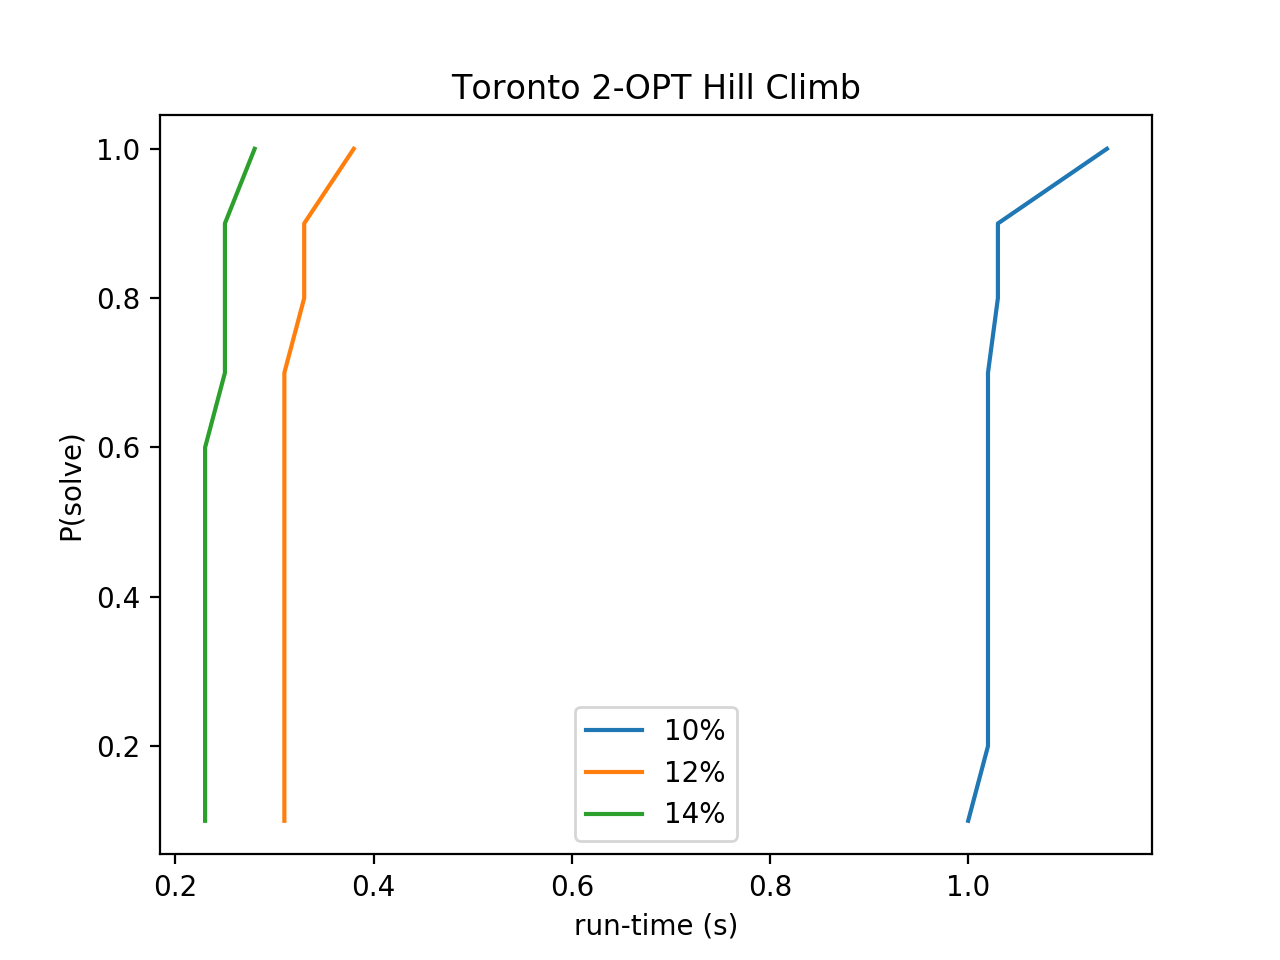
\includegraphics[scale=.5]{graphs/Toronto_LS1_QRTD.png}}
    \caption{QRTD for the 2-OPT Hill Climb on the Toronto Dataset}
    \label{fig:1}
\end{figure}

\begin{figure}[htbp]
    \centerline{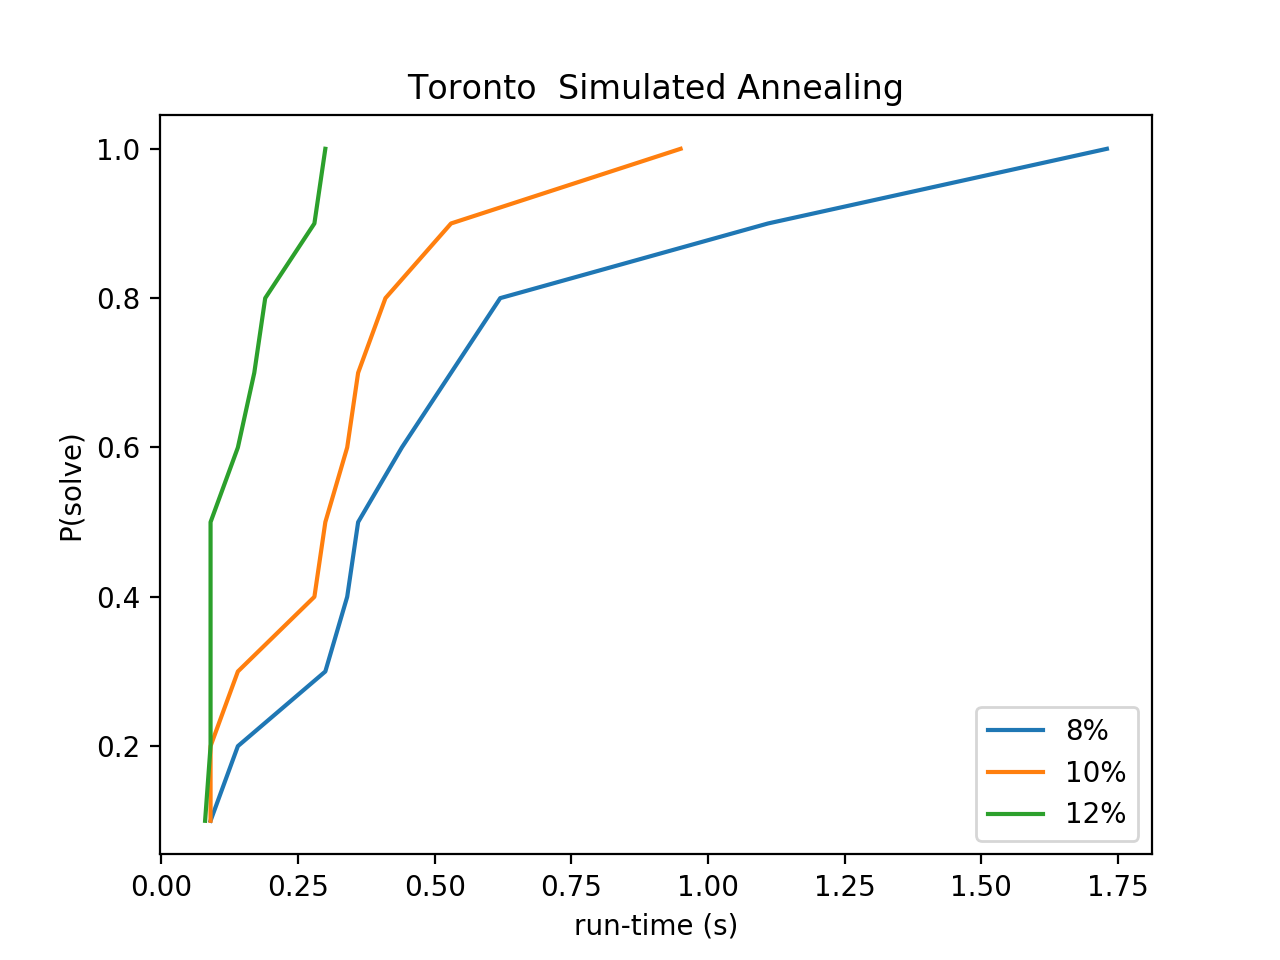
\includegraphics[scale=.5]{graphs/Toronto_LS2_QRTD.png}}
    \caption{QRTD for the Simulated Annealing on the Toronto Dataset}
    \label{fig:2}
\end{figure}

\begin{figure}[htbp]
    \centerline{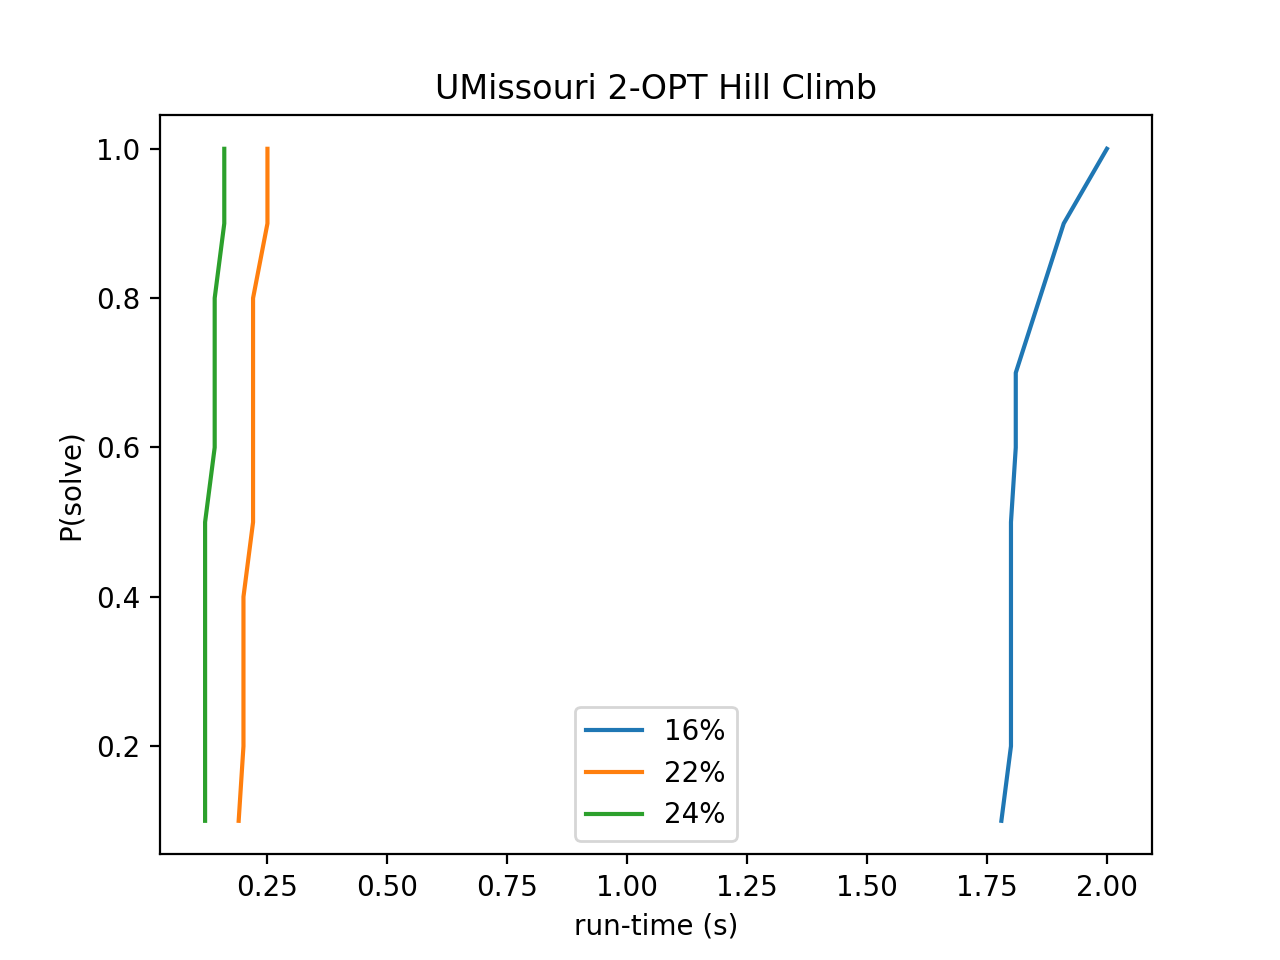
\includegraphics[scale=.5]{graphs/UMissouri_LS1_QRTD.png}}
    \caption{QRTD for the 2-OPT Hill Climb on the UMissouri Dataset}
    \label{fig:3}
\end{figure}

\begin{figure}[htbp]
    \centerline{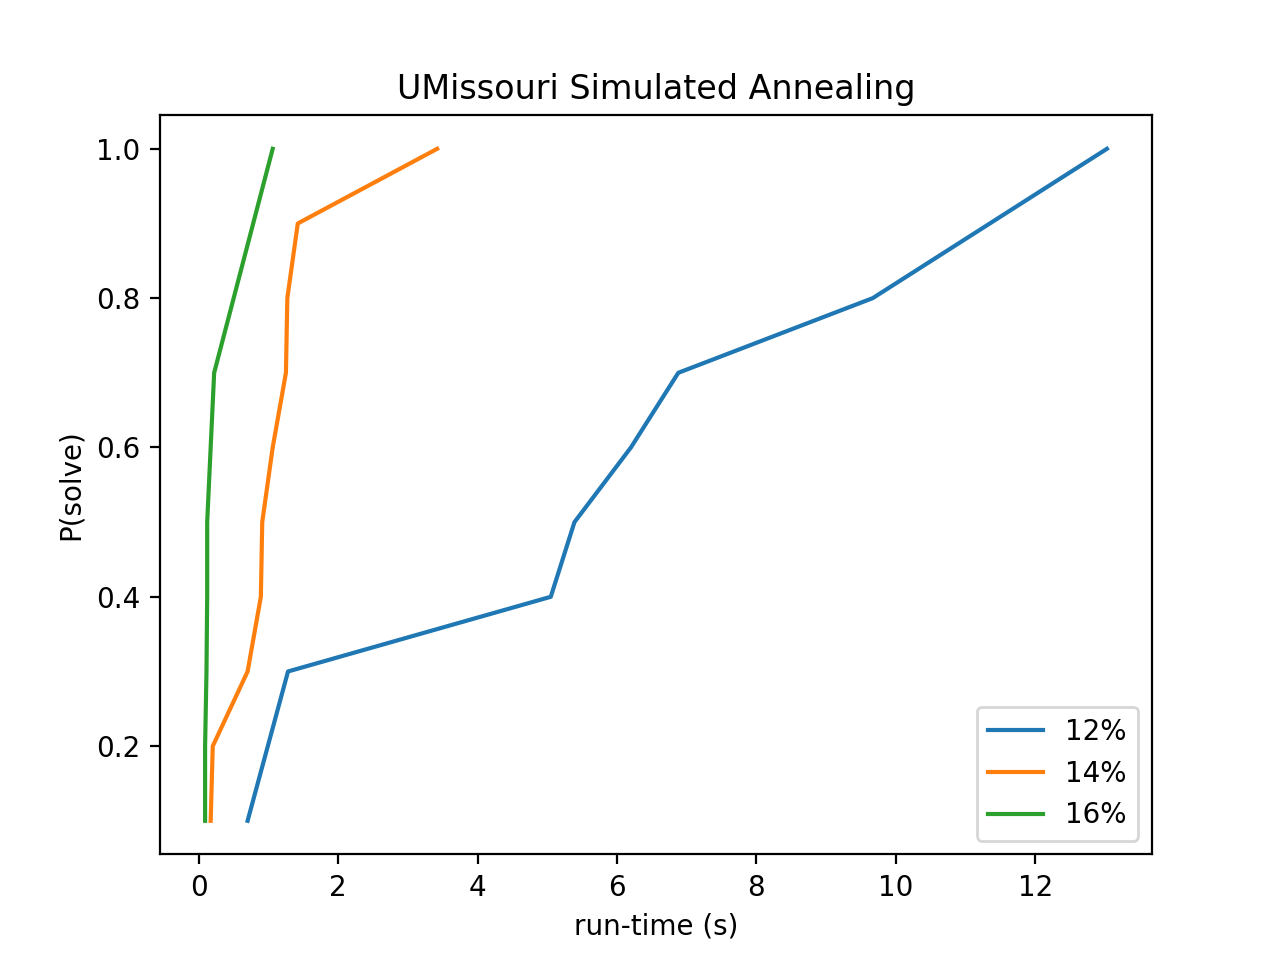
\includegraphics[scale=.5]{graphs/UMissouri_LS2_QRTD.png}}
    \caption{QRTD for Simulated Annealing on the UMissouri Dataset}
    \label{fig:4}
\end{figure}

The Qualified Runtime Distribution (QRTD) graphs for UMissouri show the major difference between the two local search algorithms, being that the 
Simulated Annealing algorithm not only performs better but is able to continue to increase its accuracy with a much higher 
probability as the algorithm continues to run. \autoref{fig:4} additionally shows that the Simulated Annealing algorithm is able 
to reach a good solution quickly, and then iterate on it initially relatively quickly. However, we see that as the solution moves 
closer to the optimal set the slope of the line begins to flatten out as the improvements take longer to make, something that intuitively makes sense 
as the set of possible solutions which are an improvement over the current solution decrease, while the search space remains stable.
\begin{figure}[htbp]
    \centerline{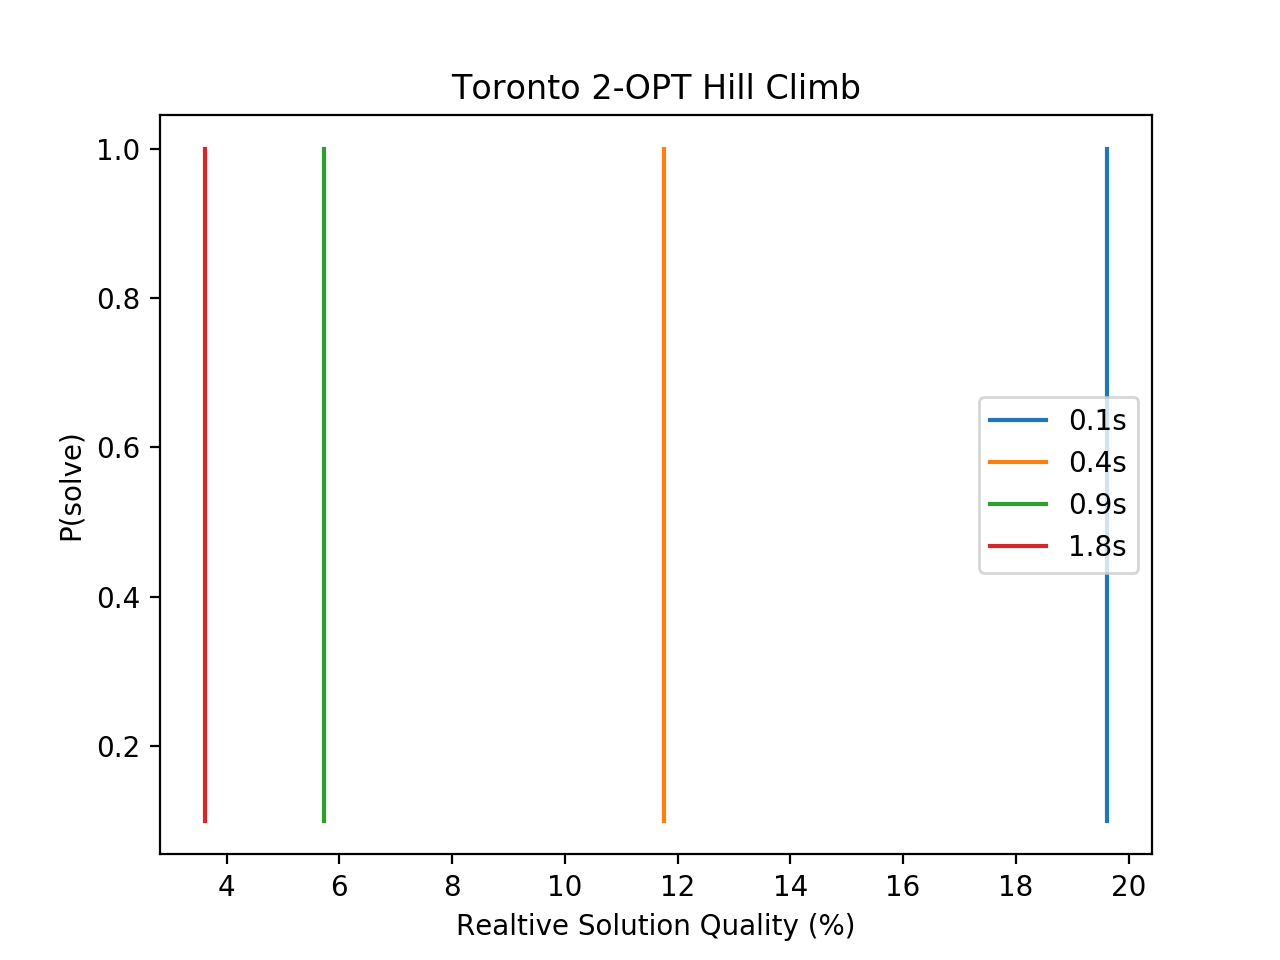
\includegraphics[scale=.5]{graphs/Toronto_LS1_SQD.png}}
    \caption{SQD for 2-OPT Hill Climb on the Toronto Dataset}
    \label{fig:5}
\end{figure}

\begin{figure}[htbp]
    \centerline{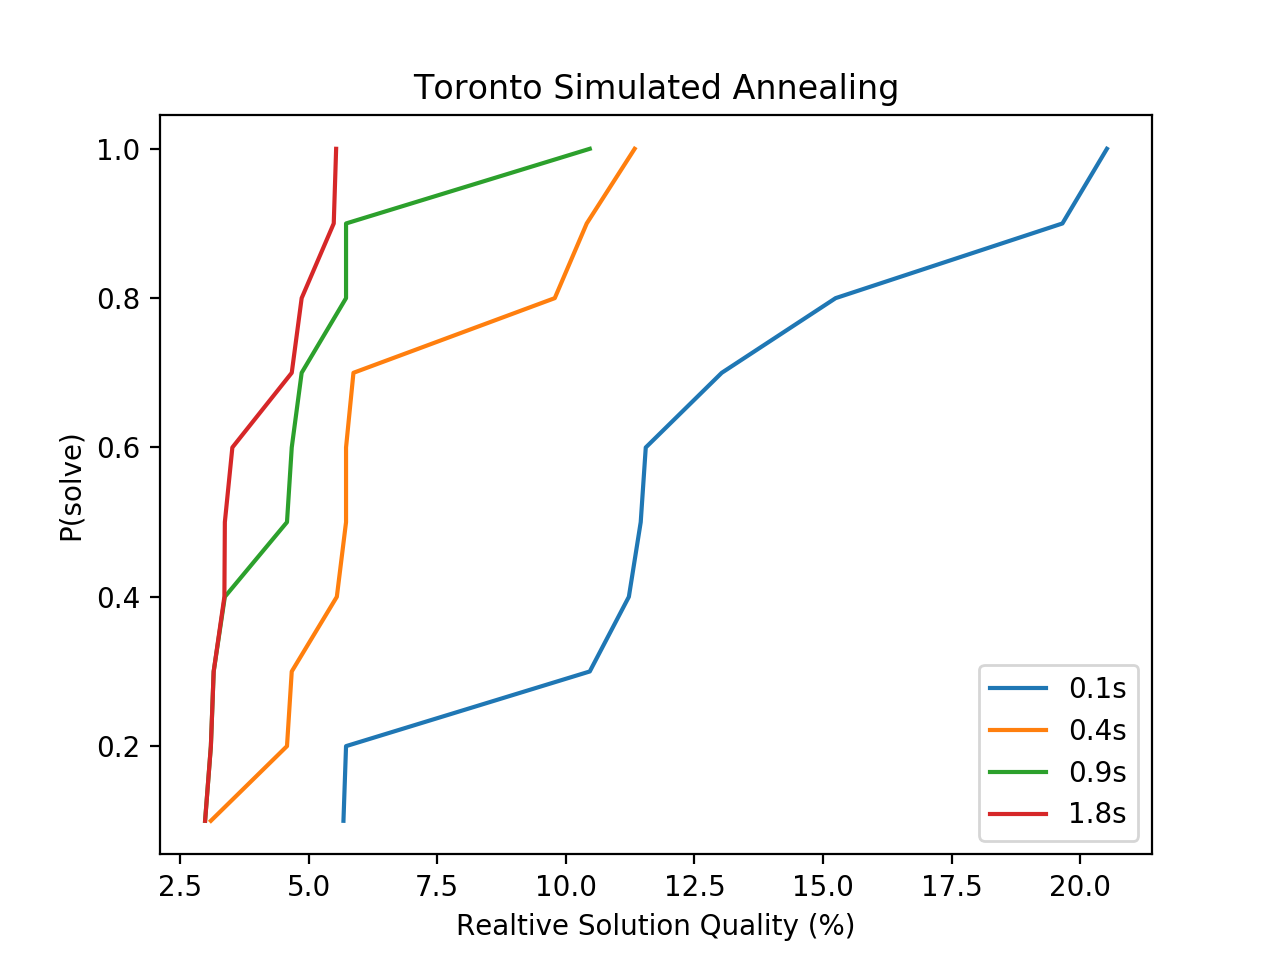
\includegraphics[scale=.5]{graphs/Toronto_LS2_SQD.png}}
    \caption{SQD for Simulated Annealing on the Toronto Dataset}
    \label{fig:6}
\end{figure}

\begin{figure}[htbp]
    \centerline{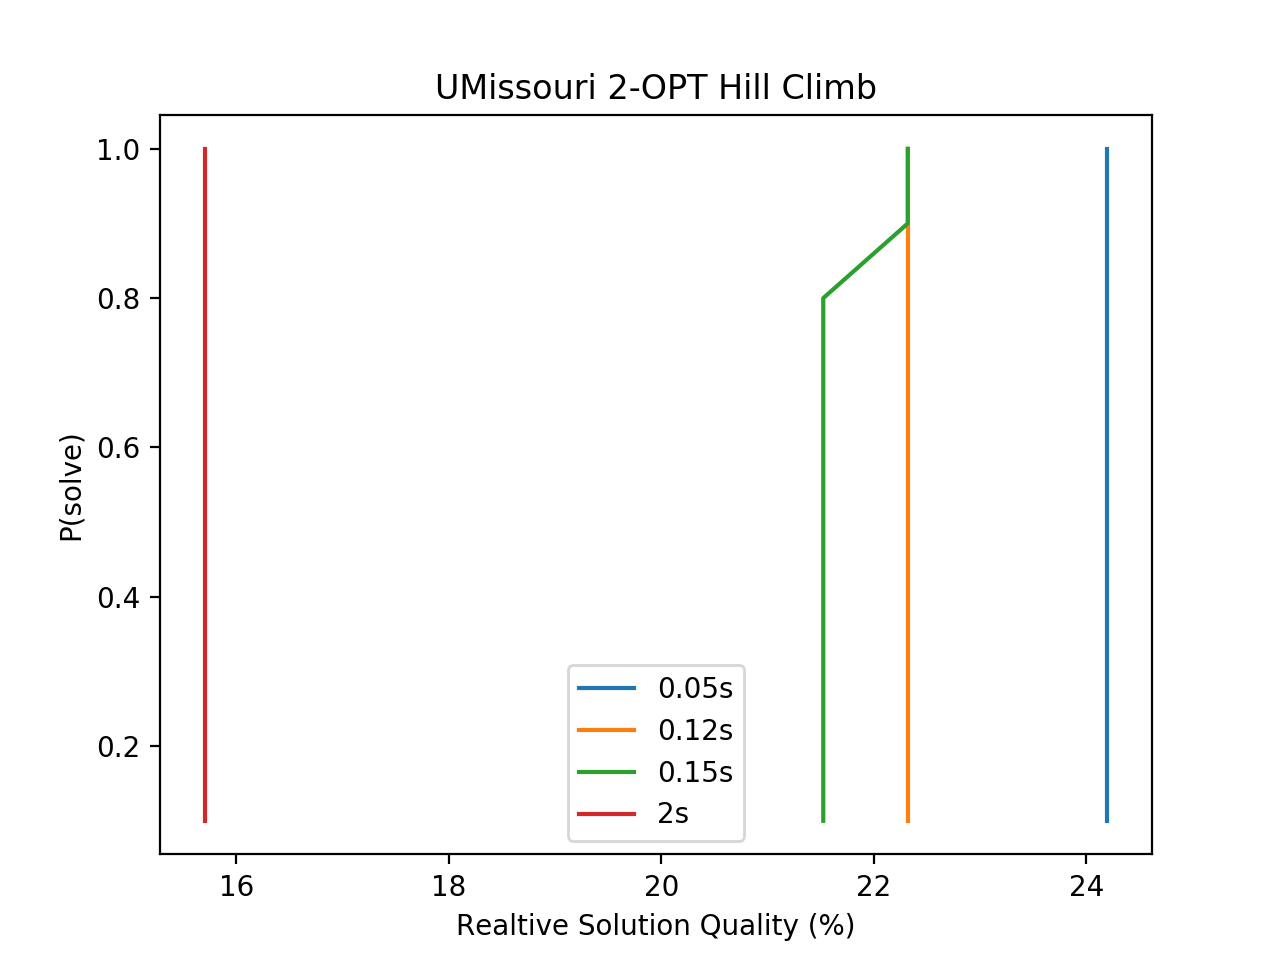
\includegraphics[scale=.5]{graphs/UMissouri_LS1_SQD.png}}
    \caption{SQD for the 2-OPT Hill Climb on the UMissouri Dataset}
    \label{fig:7}
\end{figure}

\begin{figure}[htbp]
    \centerline{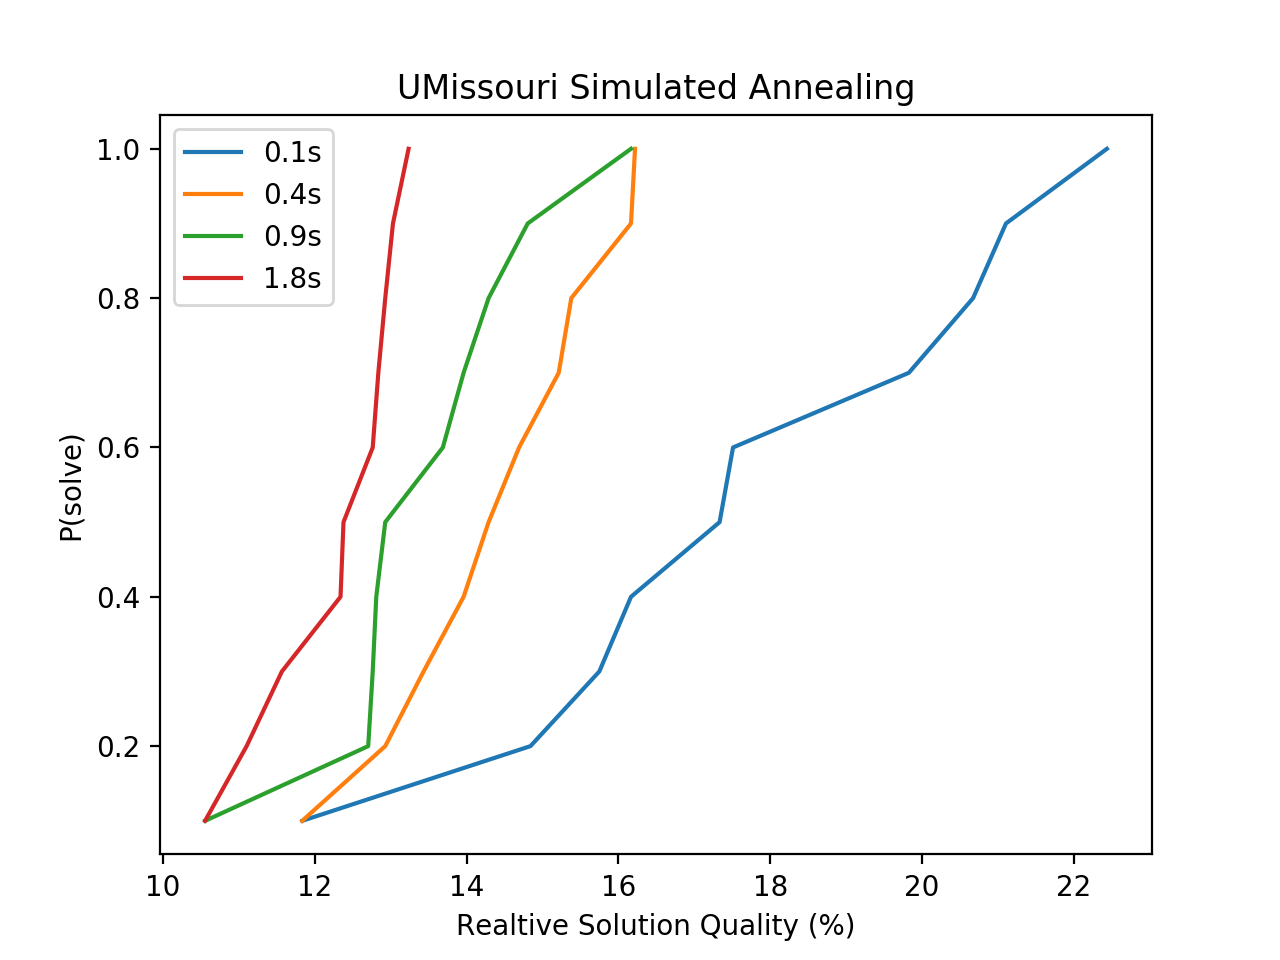
\includegraphics[scale=.5]{graphs/UMissouri_LS2_SQD.png}}
    \caption{SQD for Simulated Annealing on the UMissouri Dataset}
    \label{fig:8}
\end{figure}
The Solution Quality Distribution (SQD) graphs show the difference in the algorithms due to the 
highly random nature of the Simulated Annealing implementation in comparison to the 2-OPT Hill Climb 
implementation. When looking at \autoref{fig:5} and \autoref{fig:7} we observe that the solution qualities relative to time over all of 
the runs are almost always the same when the values are truncated to two decimal places. This is in contrast to the 
Simulated Annealing algorithms shown in \autoref{fig:6} and \autoref{fig:8} where the time is takes to reach a specified solution quality 
varies much more. Considering the different use-cases for an algorithm such as this there are situations where both cases are desireable, 
depending on whether speed or dependability are more important.
\begin{figure}[htbp]
    \centerline{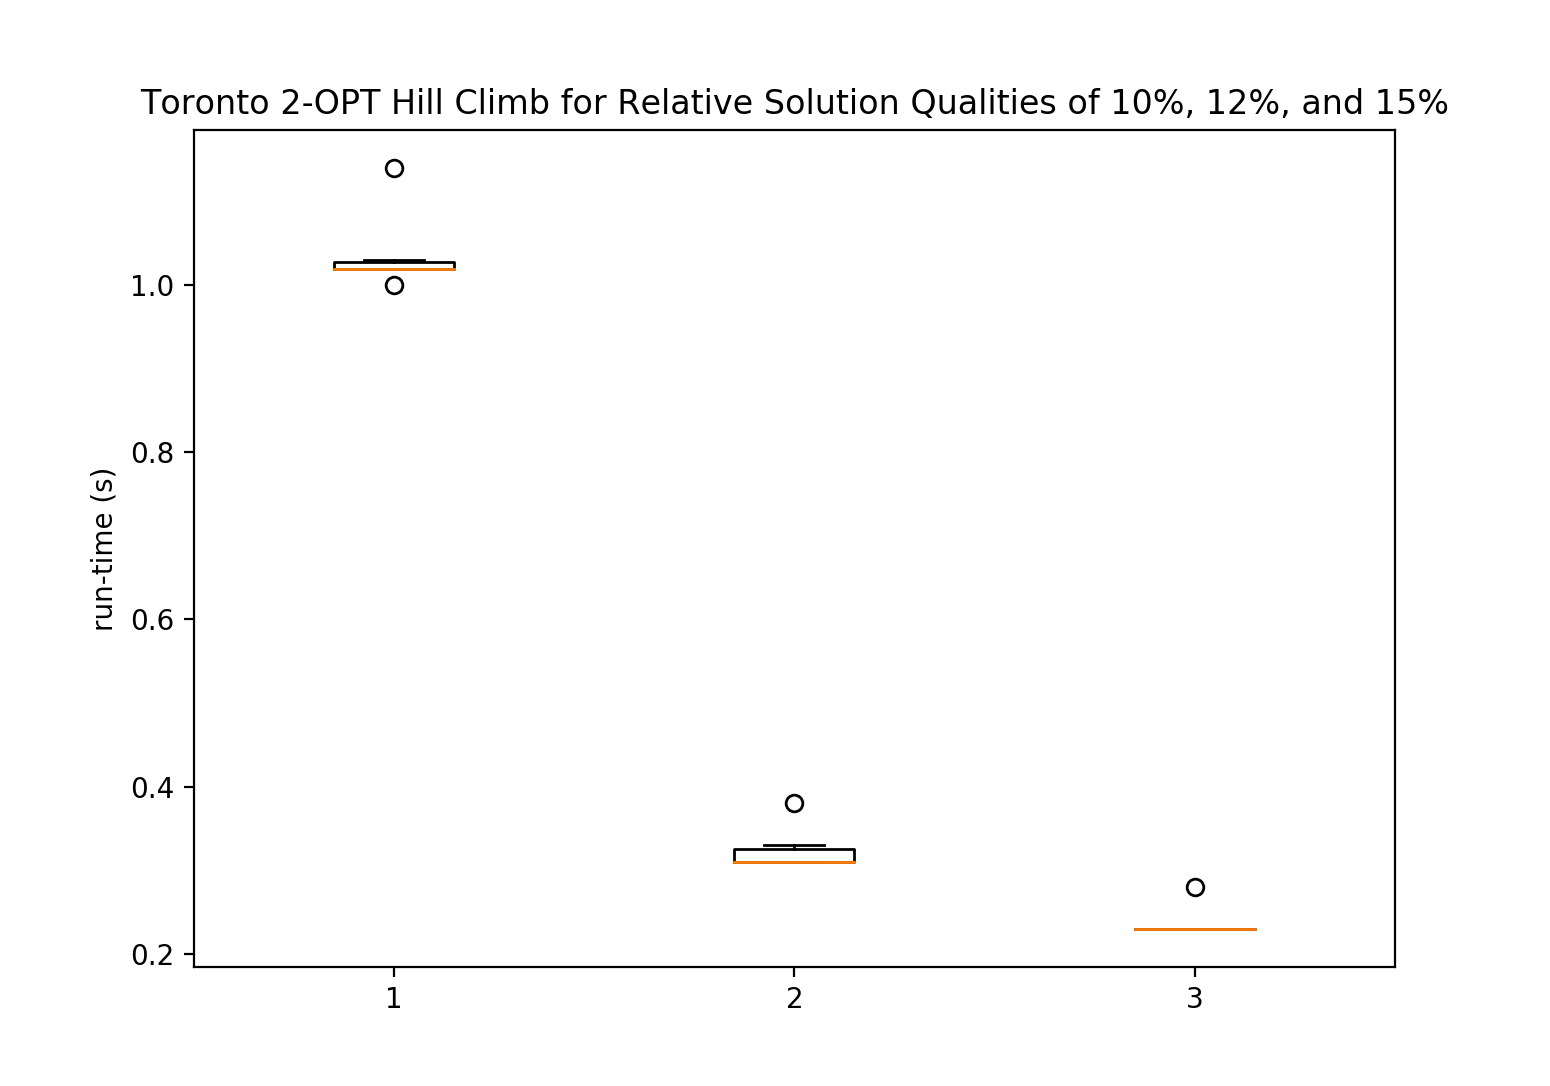
\includegraphics[scale=.5]{graphs/Toronto_LS1_Box.png}}
    \caption{Box Plot for 2-OPT Hill Climb on the Toronto Dataset}
    \label{fig:9}
\end{figure}

\begin{figure}[htbp]
    \centerline{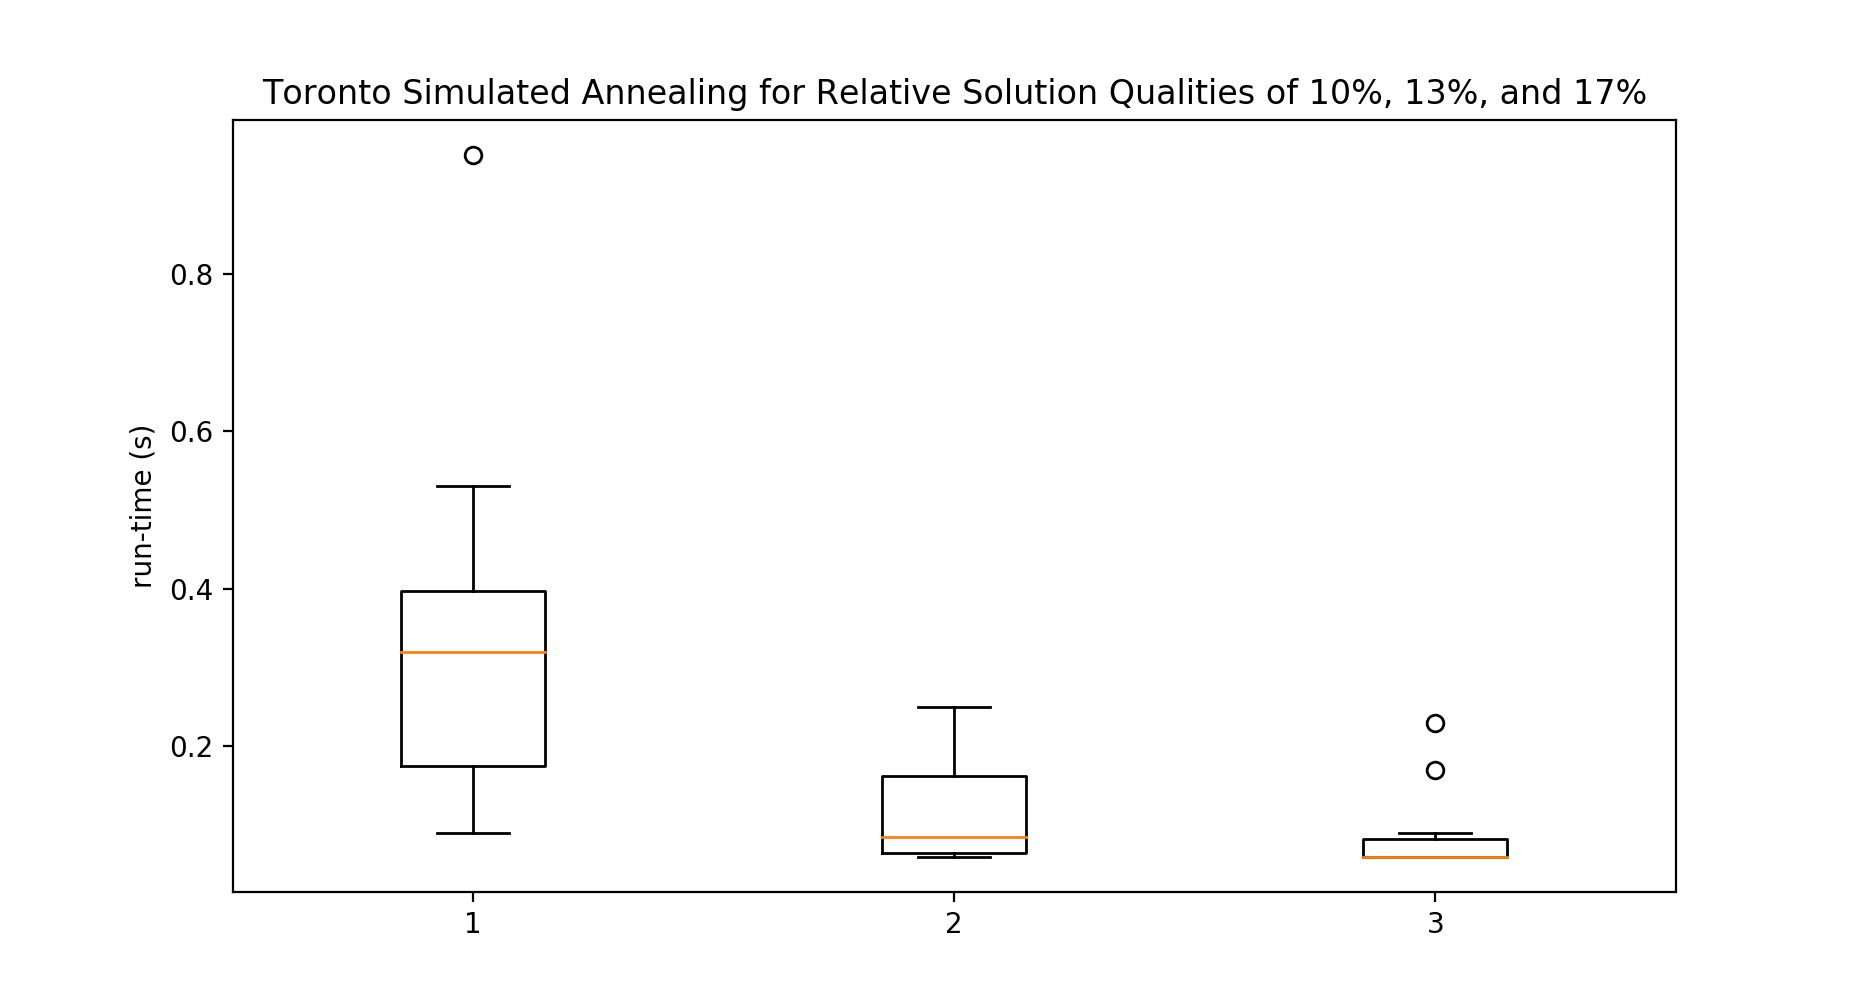
\includegraphics[scale=.5]{graphs/Toronto_LS2_Box.png}}
    \caption{Box Plot for Simulated Annealing on the Toronto Dataset}
    \label{fig:10}
\end{figure}

\begin{figure}[htbp]
    \centerline{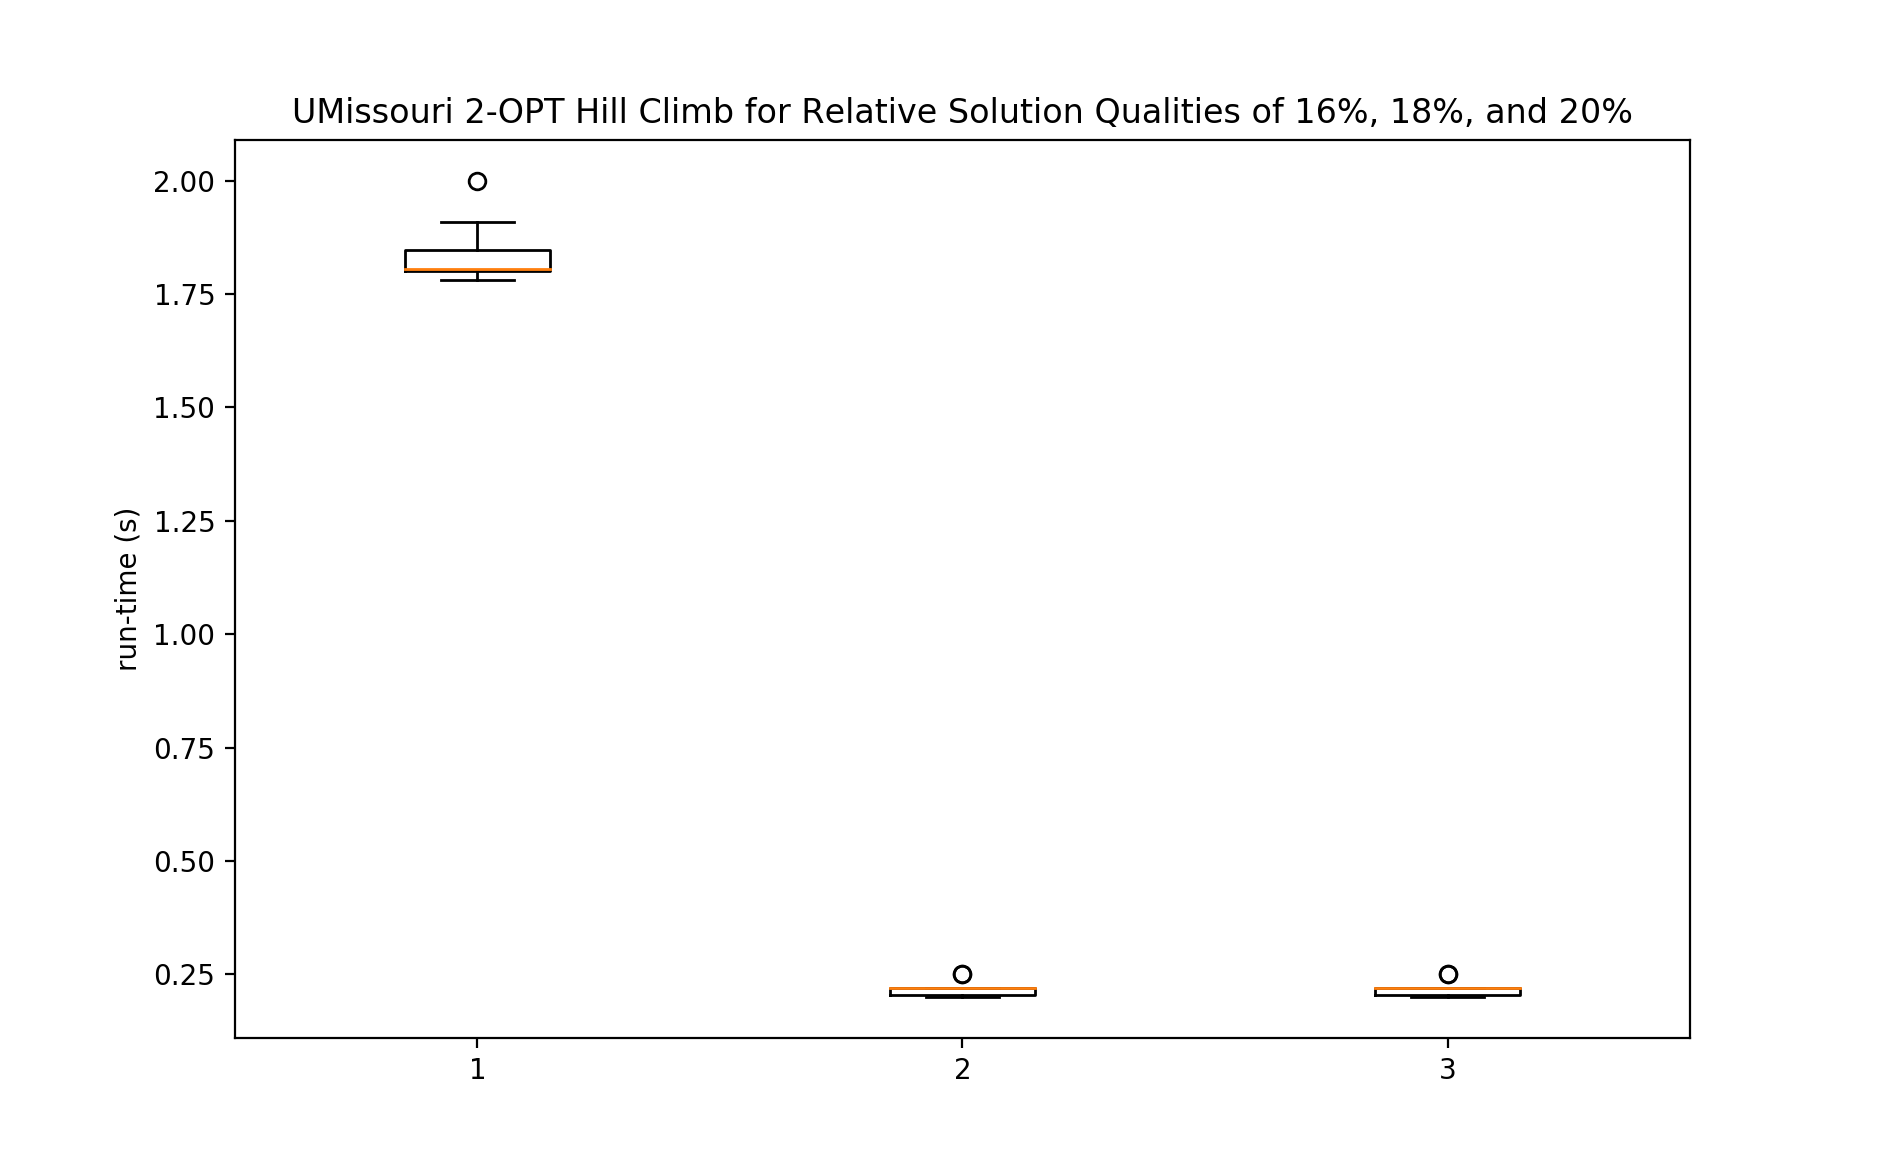
\includegraphics[scale=.5]{graphs/UMissouri_LS1_Box.png}}
    \caption{Box Plot for the 2-OPT Hill Climb on the UMissouri Dataset}
    \label{fig11}
\end{figure}

\begin{figure}[htbp]
    \centerline{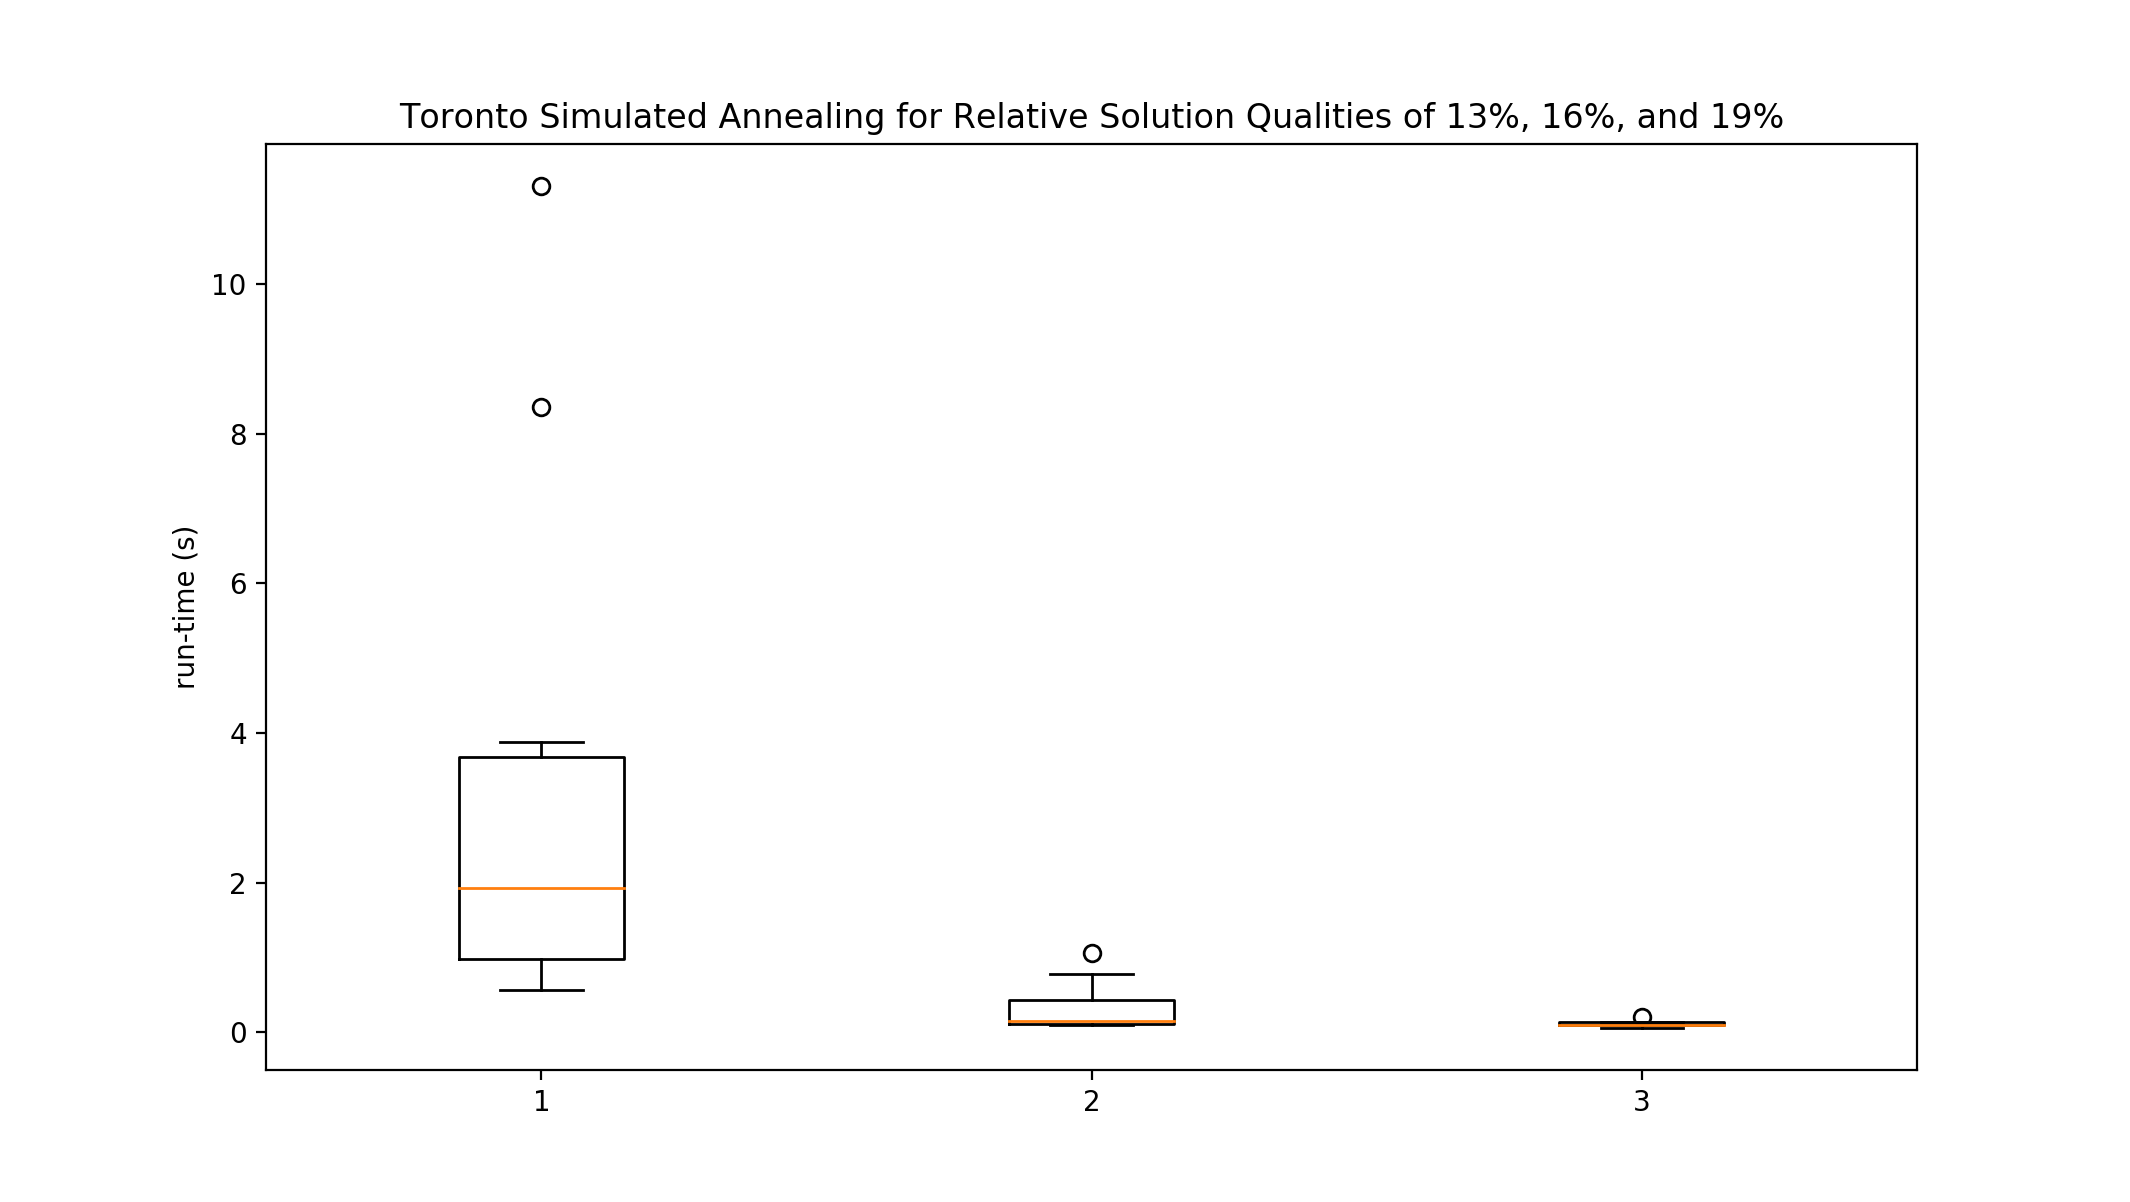
\includegraphics[scale=.5]{graphs/UMissouri_LS2_Box.png}}
    \caption{Box Plot for Simulated Annealing on the UMissouri Dataset}
    \label{fig12}
\end{figure}
The box plot detailed in \autoref{fig:10} is especially interesting with regards to the way which the run-times
change as the error of the algorithm decreases. The first box plot shows the run-times to reach a relative error of 10\%, while the third plot 
shows the run-times for a solution error of 17\%. The lower error calculations not only have greater magnitude, but also a much higher variance 
which shows not only the obvious increase in execution time but the increase in run-time variability.

 \clearpage
\section*{Discussion}
\textbf{Branch-and-Bound}\newline
\textbf{Approximation Algorithm}\newline
\textbf{Local Search} The 2-Opt Exchange and Simulated Annealing algorithms each performed relatively 
well for the majority of data-sets based on algorithm run-time versus performance. For each algorithm instance, a short
algorithm runtime was able to produce results which were in most cases within 5\% of the optimal solution. Each algorithm setup 
used a simple Greedy approximation algorithm as the initial path for local search. When testing different initial paths, the Greedy path 
proved to provide a good mix between accuracy and execution time as a strong initial solution was presented quickly by the algorithm, allowing more local 
search iterations per time-frame. The Simulated Annealing 
provided a clear benefit over the 2-opt exchange hill climbing setup however, which was due mainly to the ability of the algorithm to consider 
a broader neighborhood than the strict neighborhood that the 2-Opt exchange argument considered. To more clearly identify this, the $\alpha$ value was 
varied with a clear decrease in performance observed when the $\alpha$ value was deviated far from the eventual selection of .98 in either direction. 
This $\alpha$ value proved to have a reasonable affect on the annealing time-frame which allowed the algorithm to consider the entire search space thoroughly enough 
while still reaching a reasonable solution in a relatively short period of time. The 2-Opt algorithm struggled with a smaller neighborhood as only 2-Opt exchanges starting from 
all Greedy solutions were considered, and only those neighborhoods who provided a clear one to one improvement over the current best were used. The power of the Simulated Annealing setup 
becomes clear when looking at both of these local search algorithms as a similar 2-Opt Exchange neighborhood is considered in both, however the ability of Simulated Annealing to 
allow worse routes temporarily with the hope that they eventually lead to a more desireable solution proved to be key.
\section*{Conclusion}
As is true with any engineering design, the type of implementation that should be used when looking to solve the TSP is heavily based on the type of results that are desired. All 
of the algorithms that were tested proved optimal for various situations depending on whether or not the driving factors for the implementation were speed or accuracy of the final solution 
in relation to the optimal. For example, the Branch-and-Bound algorithm proved to be reasonable when the dataset was relatively small, time was not a factor, and the desired outcome was to obtain a solution 
close or equal to the optimal. When the solution space ballooned the branch-and-bound did not provide as good of results compared to the extra time that it took to traverse the solution space, often becoming stuck 
traversing branches which in the end proved worse or not much better than previous solutions. For these larger cases both the Simulated Annealing and 2-OPT Hill Climb algorithms performed in many cases better than the Branch-and-Bound 
algorithm in considerably less time. Had the Branch-and-Bound algorithm been given hours to run instead of the designated 10 minutes, the solution returned likely would have been much closer to optimal than the Local Search algorithms were able 
to provide. However, when compute power and time is a constraint the Local Search algorithms proved to be the optimal method for evaluating the TSP algorithm. The Approximation algorithm in all cases returned with the greatest error, something 
which is to be expected based on the algorithm implementation. However, the extremely short runtimes make the approximation algorithm reasonable when looking to computer an initial solution, or when solution error is not the most important factor to consider 
execution time is prioritized.
\bibliographystyle{ACM-Reference-Format}
\bibliography{bibfile}
\end{document}